\chapter{Extendiendo RISC-V}

Este capítulo explica los pasos seguidos para diseñar un acelerador de BNN, como se ha incluido en una CPU RISC-V y los resultados que se han obtenido al utilizarlo.

\section{Diseño del acelerador}

Como se ha explicado en secciones previas, la sección del algoritmo mas importante a optimizar es el muestreo de distribuciones gaussianas. Para ello se va incluir un GRNG como una nueva unidad funcional (UF) en la CPU RISC-V base. Sarwar Malik \emph{et al.} \cite{clt_grng} propusieron un diseño basado en el TCL que añadía un componente corrector para reducir el error de muestreo de las colas de la distribución. Como también se ha mostrado previamente, no es necesaria una gran precisión a la hora de muestrear distribuciones, por lo que se va a diseñar un GNRG basado en la suma de 12 distribuciones uniformes sin bloque corrector.

\subsection{Generación de números pseudoaleatorios uniformes}

Para generar números pseudoaletorios uniformes se ha utilizado un componente hardware llamado \textit{\textbf{L}inear \textbf{F}eedback \textbf{S}hift \textbf{R}egister} (LFSR). Se basan en un circuito de retroalimentación y un registro de estado. El circuito de retroalimentación es un conjunto de puertas XOR que implementan un polinomio generador. Dado un registro de estado de $n$ bits, si el polinomio puede producir $2^n-1$ valores antes de empezar a repetir la secuencia entonces la secuencia es máxima. Alfke \cite{lfsr_poly} recopiló una lista de polinomios generadores para secuencias máximas para varios tamaños de registros de estado.

La desventaja de este tipo de LFSR es que no pueden generar más de un bit con baja correlación entre muestras.

%\boxtext{\begin{itemize}
%    \item solo pueden generar un bit con baja correlacion, para eso se utilizan look-ahead lfsr, que genera varios por que avanza varios ciclos mediante un circuito mas complejo
%    \item cita al paper y a las ecuaciones para generar las matrices \cite{look_ahead_lfsr_base, look_ahead_lfsr_design}
%    \item explicar implementacion de script python que genera codigo vhdl para una configuración arbitraria de lfsr
%\end{itemize}}

\subsection{Generador de números pseudoaleatorios gaussianos}

\todo Suma de 12 valores de 12 bits, todos considerados en escala $2^{12}$ para que representen valores entre 0 y 1 (muestras uniformes 0,1). se segmenta para evitar problemas con el reloj, solo afecta al cambiar la semilla que hay 4 valores que hay que tirar, esto lo hace automaticamente el acelerador pero hay que dejar al menos 4 ciclos sin consumir datos

\begin{figure}[h]
    \centering
    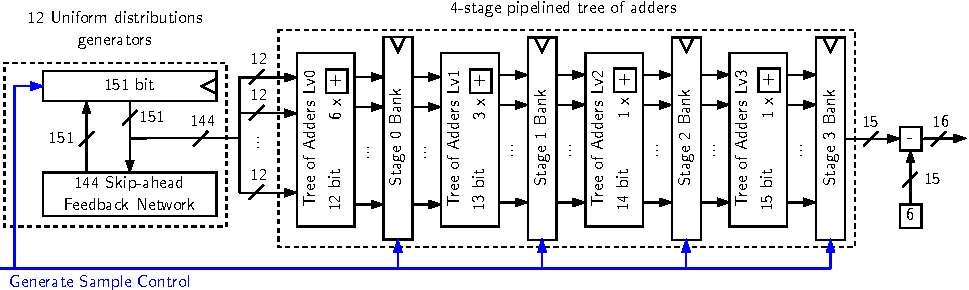
\includegraphics[width=\textwidth]{Imagenes/grng.pdf}
    \caption{\todo}
    \label{fig:aa}
\end{figure}

\section{Modificaciones al procesador}

Se añade como una unidad funcional extra en execution. Esto permite hacer una modificacion minima al procesador, actualizar decode y actualizar el selector de resultado que avanza a la siguiente etapa.

Otra opción es añadirlo como un periférico mapeado en memoria que se acceda mediante instrucciones load store. En este caso impone problemas con los consumidores a distancia 1 lo implica perdida de rendimiento. Generalmente el acceso a memoria tiene que pasar por circuitos mas complejos que añaden retardo (MMU) (en nuestro caso no ocurre).

\begin{figure}[h]
    \centering
    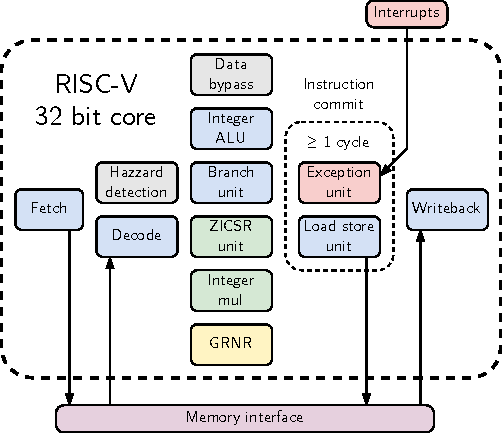
\includegraphics[width=0.9\textwidth]{Imagenes/riscv_core_extended.pdf}
    \caption{\todo}
    \label{fig:bb}
\end{figure}


\subsection{Actualizar el compilador}
\todo

Como hemos añadido instrucciones nuevas para poder utilizaras desde codigo de alto nivel como C hay que actualizar el compilador.

\begin{itemize}
    \item \texttt{setseed rs1} cambia la semilla por el valor del registro \texttt{rs1}.
    \item \texttt{genum rd} genera una muestra de $\mathcal{N}(0,1)$ y la guarda en los 16 bits mas altos del registro \texttt{rd}. Eso implica que la muestra está en coma fija en escala $2^{12 + 16}$.
\end{itemize}

Para actualizar el compilador hay que cambiar hay que cambiar el código fuente de gcc. Modificar los ficheros \texttt{riscv-gnu-toolchain/riscv-binutils/opcodes/riscv-opc.c} y \texttt{riscv-gnu-toolchain/riscv-binutils/opcodes/riscv-opc.h}. Para ello hay que definir la codificación de las instrucciones mediante máscaras y valores para validar la mascara.
\begin{table}[H]
    \centering
    \caption{Caption}
    \label{tab:my_label}
    \begin{tabular}{cccccccc}
        &  funct7 &  rs2 &  rs1 &  funct3 &  rd &  opcode & \\
        setseed &  0000000 &  xxxxx &  xxxxx &  000 &  00000 &  0001011 & \\
        MASK &  1111111 &  00000 &  00000 &  111 &  11111 &  1111111 & 0xFE007FFF \\
        MATCH &  0000000 &  00000 &  00000 &  000 &  00000 &  0001011 & 0xB\\
        genum & 0000000 & 00000 & 00000 & 001& xxxxx & 0001011 &\\
        MASK & 1111111 & 11111 & 11111 & 111& 00000 & 1111111 & 0xFFFFF07F\\
        MATCH & 0000000 & 00000 & 00000 & 001& 00000 & 0001011 & 0x100B\\
    \end{tabular}
\end{table}

\begin{itemize}
\item campos \texttt{/* name, xlen, isa, operands, match, mask, match\_func, pinfo.  */}
\item “d” is for destination
\item “s” is for source register 1
\item “t” is for source register 2
\end{itemize}

\texttt{\{"setseed", 0, INSN\_CLASS\_I, "s,t", MATCH\_SETSEED, MASK\_SETSEED, match\_opcode, 0\}}

\texttt{\{"genum", 0, INSN\_CLASS\_I, "d", MATCH\_GENUM, MASK\_GENUM, match\_opcode, 0\}}

Luego estas instrucciones se pueden utilizar mediante inlines de ensamblador.

\begin{verbatim}
    
\end{verbatim}

\section{Análisis de resultados}

\subsection{Análisis de coste}
\todo pequeña introduccion de que es una FPGA quizas aqui

implementacion en FPGA utilizando Xilinx ZCU104 FPGA board: 240 Look-Up Tables (LUT) and 320 Flip-Flops (FF). Power measurements where obtained using the power report of Vivado Design suite. %, which implies a 9.86 and a 16.65\% increment for LUT and FF, respectively, over our small base CPU. 
This cost includes the GRNG and the modifications of the CPU instruction decoding and the data pipeline. These modifications have no impact on the 100 MHz clock, and only increase the power consumption by 0.65\%. Therefore, the reduction in energy consumption is almost identical to the performance gain. 

\begin{table}[ht]
\centering
\caption{FPGA resource utilization and power consumption of the baseline RISC-V CPU and the GRNG extension.}
\label{tab:riscv_fpga_utilization}
\begin{tabular}{lrrr}
\hline
& \multicolumn{2}{c}{\textbf{Resource Utilization}} & \textbf{Utilization \%}\\
\textbf{Type} & \textit{Base CPU} & \textit{GRNG Extension} & \textit{Extended CPU}\\ \hline
LUT	        & 2435 & 240 & 1.16 \\
Flip-Flop	& 1922 & 320 & 0.49 \\
BRAM	    & 16   & 0 & 5.13 \\
DSP	        & 12   & 0 & 0.69 \\ \hline
 & \multicolumn{3}{c}{\textbf{Power consumption (W)}} \\
\textbf{Type} & \textit{Base CPU} & \textit{GRNG Extension} \\ \hline
Dynamic & 0.023 & 0.004 \\
Static & 0.593 & 0 \\ \hline
\end{tabular}
\end{table}

